\documentclass[./Report_main.tex]{subfiles}
\graphicspath{ ./ }
\begin{comment}
If you want a box around your answer and that answer is an
equation then use \boxed{$$ equation $$} 

if you want to indent a block of text:
\begin{adjustwidth}{cm of right indent}{cm of left indent}
% paragraph to be indented
\end{adjustwidth}

if you just want one indent for one line 
use \indent per intended indent per line

A sections numbers automatically, so if the number of 
the problem is out of order it would be easier to 
just indent and bold the sections and subsections
and not use the \section{} kind of commands

\newpage makes a new page

$normal math mode$
$$Special math mode$$

to include an image use
\includegraphics{image_name}
image_name is the file name (.png) without the extension. The file
name cannot have any spaces or any periods other than the one before
the file extension.

To include a codeblock use
\begin{lstlisting}
ExampleCode(blah, blah)
{
	it does tabbing and everything;
	for (coloring of major languages like java){
		add the folloing to the \lstset tuple:
			language=<name_of_language>;
	}
}
\end{lstlisting}

\end{comment}


\begin{document}

%\tableofcontents

%\thispagestyle{empty}
%\newpage
% If you want to change how the subsubsection's are numbered
%\renewcommand{\thesubsection}{\thesection.\alph{subsection}.} 

%\setcounter{page}{0}
\chapter{Architectural Design}
\section{block diagram}
\subsection{Translation process}
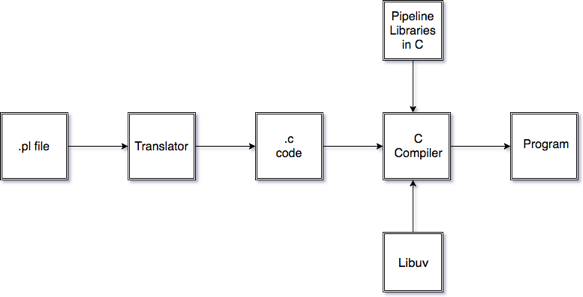
\includegraphics[scale = 0.5]{block_1.png}\\

The translation process begins with a .pl, which enters the translator and exits a .c file. This .c file is passed into the C compiler, which makes use of libraries written in C specifically for
Pipeline, as well as the Libuv library. Out of the C compiler comes a binary file capable of executing.
\subsection{Inside the translator}
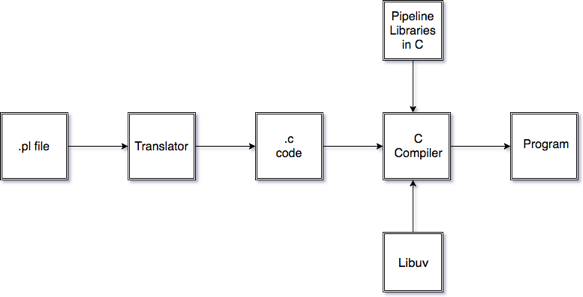
\includegraphics[scale = 0.5]{block_2.png}\\

The translator consists of a scanner and parser which deconstruct and build a pipeline file into an abstract syntax tree, which is then semantically checked to output a sematic AST, which is then
traversed by a codegen to print out a .c file.
\section{interface}
The components above map to files in the following way:\\
\begin{verbatim}
scanner             ->  scanner.mll
parser              ->  parser.mly
codegen             ->  codegen.ml
semantic checker    ->  semant.ml
ast                 ->  ist.ml
\end{verbatim}

\section{libuv}
The details of libuv are beyond this report, and can be found online (http://docs.libuv.org/en/v1.x/). However, what is important is the way the Pipeline language makes use of libuv. Pipeline operates by a singly-threaded, asynchronous, event-driven paradigm. That is, the behavior of a Pipeline program can be modeled by a single thread with a central scheduler deciding what will run on the thread at any given time. When blocking functions are contained inside pipes, the scheduler
makes sure the single thread does not block.\\\\
Libuv is essential to this paradigm. The C library handles scheduling of different blocking functions, keeping the main thread running, and thereby increasing the efficiency of event-driven programs. When a pipe is declared, we wrap the entire body of the pipe in a C function, and pass this C function to the libuv event loop using the function uv\_queue\_work. This tells libuv to run the wrapper function until it blocks, at which point it will move it off the main thread to make way
for other functions added to the event loop in an identical manner.\\\\
A special case involves routing in Pipeline. When a pipe contains a listen (a pipe can only contain one listen) and any number of http routing handler registers, we generate in C a set of functions unique to each listen. This set of functions is as follows:\\\\
\begin{verbatim}
work                    ->      normally contains the body of a pipe;
                                when a listen is in the pipe, contains 
                                only listen(string ip, int port)
listen                  ->      registers a TCP listener for the specific IP and port
on_new_connection       ->      callback called when a new TCP connection is initiated
on_read                 ->      callback called when data reading begins from the connection
post_listen             ->      contains the remainder of the body of the pipe 
                                less routing functions; also contains a set of if statements 
                                matching HTTP method and route to route handlers
\end{verbatim}
%\section{}
%\subsection{Identifiers}
%\subsubsection{}
%\subsection{subsection}
%\subsubsection{subsubsection}
\end{document}

